\chapter{\acl{ft} Sensor Compensation}
\label{chapter:ft-sensor-correction}

% ADD: Dar introdução ao capítulo
% \par In this chapter... (\textbf{dar a outline do capítulo})

\section{\ac{ft} Sensor Correction}

\par To achieve the tasks that require physical contact between the human and the cobot, the UR10e built-in \ac{ft} sensor, located at its \ac{eef} will be extensively used. Its technical specifications can be found in \autoref{tbl:ur10e-specs}. There are two ways of interfacing with the sensor, both of them managed by the URControl controller. One of them is through URScript commands, with \textit{get\_tcp\_force()} used for obtaining the \ac{ft} values at the \acs{tcpr}, and \textit{zero\_ftsensor()} that zeroes the \ac{ft} measurement by subtracting the current measurement from the subsequent. The other, is using the \ac{ur} \ac{ros} Driver which publishes the \ac{ft} measurement in the \textbackslash\textit{wrench} topic at 500Hz, and exposes the \textbackslash\textit{zero\_ftsensor} service. Relevant to this matter, the Polyscope interface has a configuration parameter used to describe the weight coupled to the \acs{tcpr}, called Payload. It is composed of mass, in Kg, and \ac{cog}, in cartesian coordinates, and their effect on the \ac{ft} measurement will be later demonstrated in \autoref{ssec:ft_internal_comp}.

\subsection{Noise Filtering}

% LER: Signal Processing and Application of Six-axis Force/Torque Sensor Integrated in Humanoid Robot Foot

\par As seen in \autoref{tbl:ur10e-specs}, the \ac{ur10e} \ac{ft} sensor has a reported resolution of 2 N on force, and 0.02 Nm on torque measurements. The 2 leftmost graphs of \autoref{fig:ft_sensor_filter} demonstrate that this fact is due to the noise generated by the hardware of the sensor. 

\begin{equation}
    \mathbf{W_{fil}} = (1-\alpha)W_n + \alpha \left(\frac{W_n + W_{n-1}}{2}\right)
    \label{eq:wrench_filter}
\end{equation}

% Moving Average Filter
% https://maker.pro/arduino/tutorial/how-to-clean-up-noisy-sensor-data-with-a-moving-average-filter#:~:text=What%20is%20a%20Moving%20Average,frequency%20information%20from%20the%20output.
% Low Pass Filter
% https://dobrian.github.io/cmp/topics/filters/lowpassfilter.html#:~:text=Introduction,lower%20frequencies%20to%20pass%20through.&text=In%20a%20digital%20signal%20received,contain%20occasional%20spurious%20incorrect%20values.

\par The chosen way of dealing with the noise is to apply a \ac{lpf} to the raw measurements. \autoref{eq:wrench_filter} defines a 2\textsuperscript{th} order \ac{fir} filter with an average component added to it. Other types of \acp{lpf} were also considered, such as a \ac{maf} but the results were not satisfactory.

\par A \ac{ros} node with the purpose of filtering the raw measurements was developed. It subscribes to the \textbackslash \textit{wrench} topic, filters each value with \autoref{eq:wrench_filter} and publishes them in the \textbackslash \textit{wrench\_filtered} topic. The $\alpha$ parameter can be changed in real time using the \ac{ros} dynamic reconfigure tool. Tests showed that an $\alpha = 0.2 $ was satisfactory for noise reduction without major delay impact on the measurements. Results of this filtering technique can be observed in the rightmost graphs of \autoref{fig:ft_sensor_filter}.

\begin{figure}[h]
    \centering
    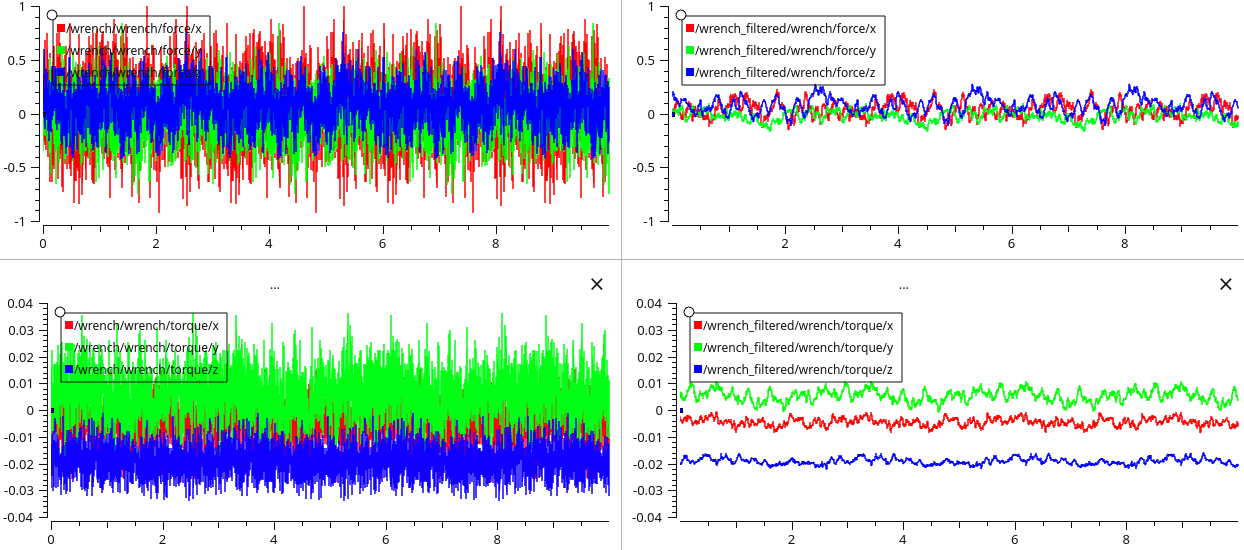
\includegraphics[width=0.9\linewidth]{figs/chp3/ft_sensor_filter.png}
    \caption{Comparison of raw and filtered \ac{ft} measurements}
    \label{fig:ft_sensor_filter}
\end{figure}


\subsection{Observed Behavior}

\par Further experiments with the \ac{ft} sensor measurements showed a couple of unexpected behaviors described in the following subsections.

\subsubsection{Wrist3 Joint Positional Variation}

\par The \ac{ft} measurements present variations relative to the position of the Wrist3 joint. \autoref{fig:w3_problem} shows a simple real time test where the \ac{eef} is fixed in a random pose, and the Wrist3 joint is rotated from \ang{-360} to \ang{360}. The \ac{ft} measurements present clear variations that can reach 8N of difference from the correct value, which should be 0N the entire test since the \ac{eef} has no tool or weight coupled to it. Changing the pose of the \ac{eef} presents the same results. 

\begin{figure}[h]
    \centering
    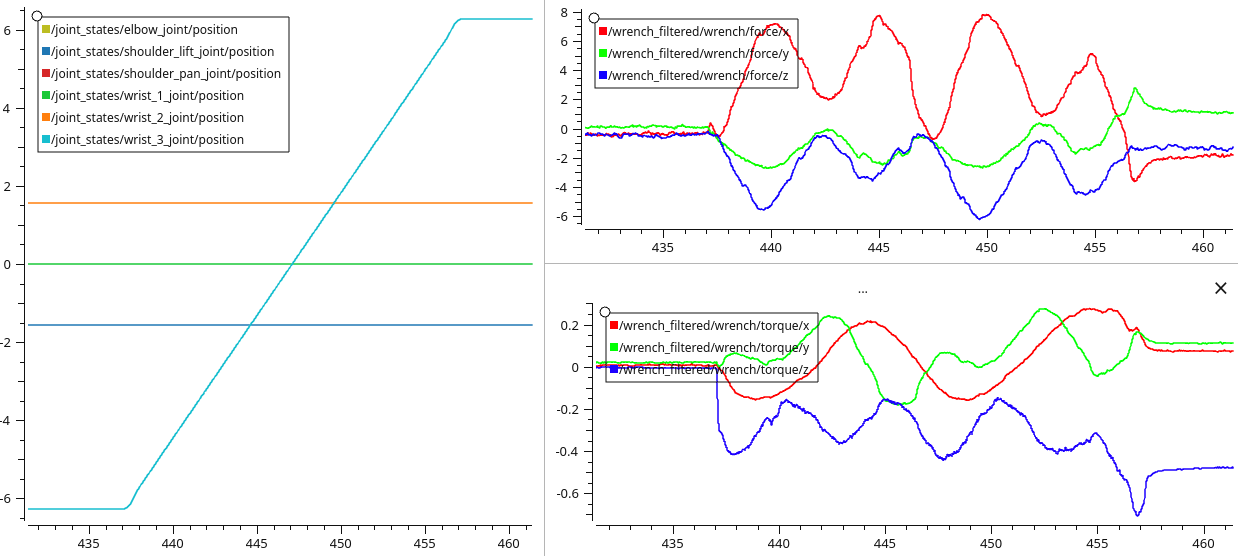
\includegraphics[width=0.9\linewidth]{figs/chp3/wrist_3_problem.png}
    \caption{Real time test of the variation on \ac{ft} relative to the position of the Wrist3 joint}
    \label{fig:w3_problem}
\end{figure}

\par This presents a problem for the accuracy of the \ac{hg} and object manipulation tasks since an error of 8N is significant. \autoref{ssec:w3_solution} demonstrates the proposed solution for this problem.

\subsubsection{Temporal Drift}

\par When the robot is left still for long periods of time, the values of force change linearly with time, as much as $0.2\si{N}/\si{min}$. It might not seem a significant value, but if an \ac{hg} task were to be activated, by letting the robot stand still for a couple of minutes, it would start moving on its owm. A recording of force values over a period of 10 minutes, with a step of 200ms is shown in \autoref{fig:ft_sensor_drift}. 

\begin{figure}[h]
    \centering
    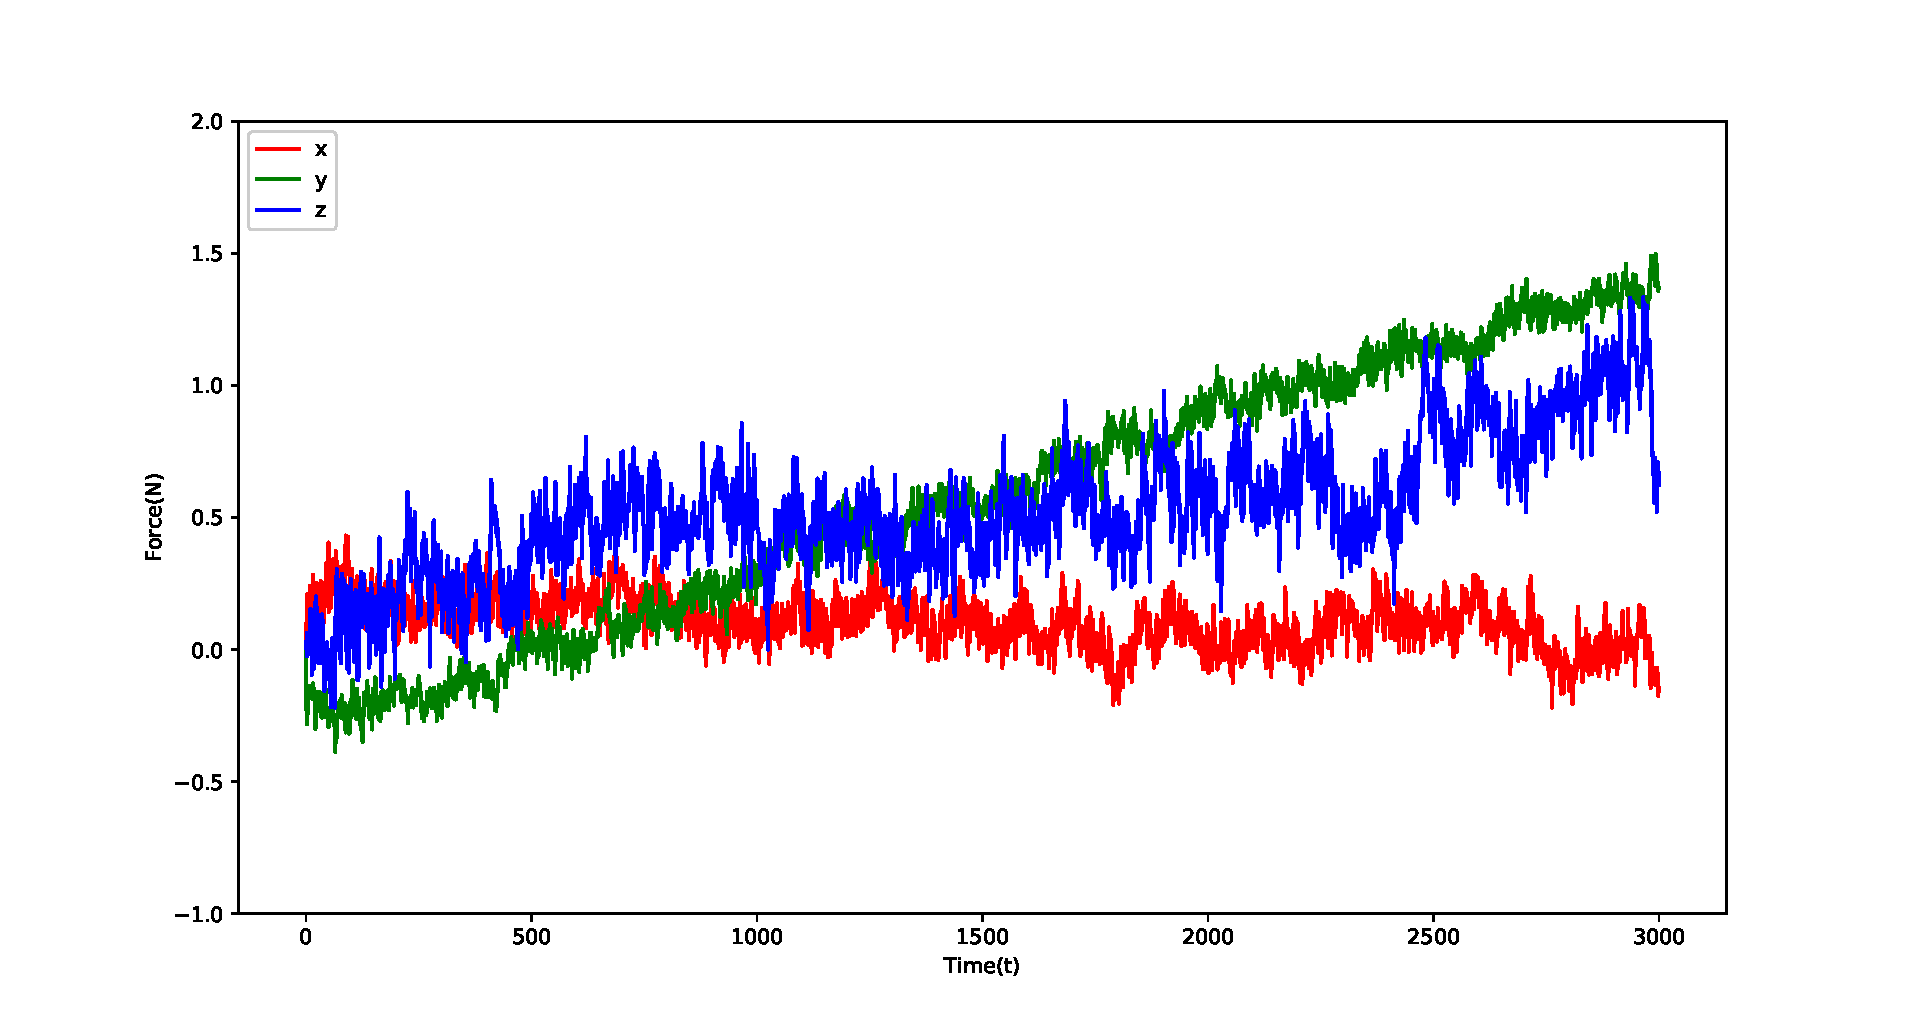
\includegraphics[width=0.8\linewidth]{figs/chp3/ft_sensor_drift.pdf}
    \caption{Variation of \ac{ft} relative to time}
    \label{fig:ft_sensor_drift}
\end{figure}

\par Using the zero\_ftsensor in a recurring, timely manner would fix this problem but raise the issue on when to do so, since it might also erase important \ac{ft} measurements needed for the executing task.

\subsubsection{Variations caused by appliying \ac{ft}}

\par Applying high amounts of external \ac{ft} to the sensor, will result in a variation on the measurements after its no longer applied. This behavior can be seen in \autoref{fig:ft_sensor_pushes} where every time there is a strong interaction with the \ac{eef}, the subsequent values of \ac{ft} present variations as high as 3N and 0.3Nm.

\begin{figure}[h]
    \centering
    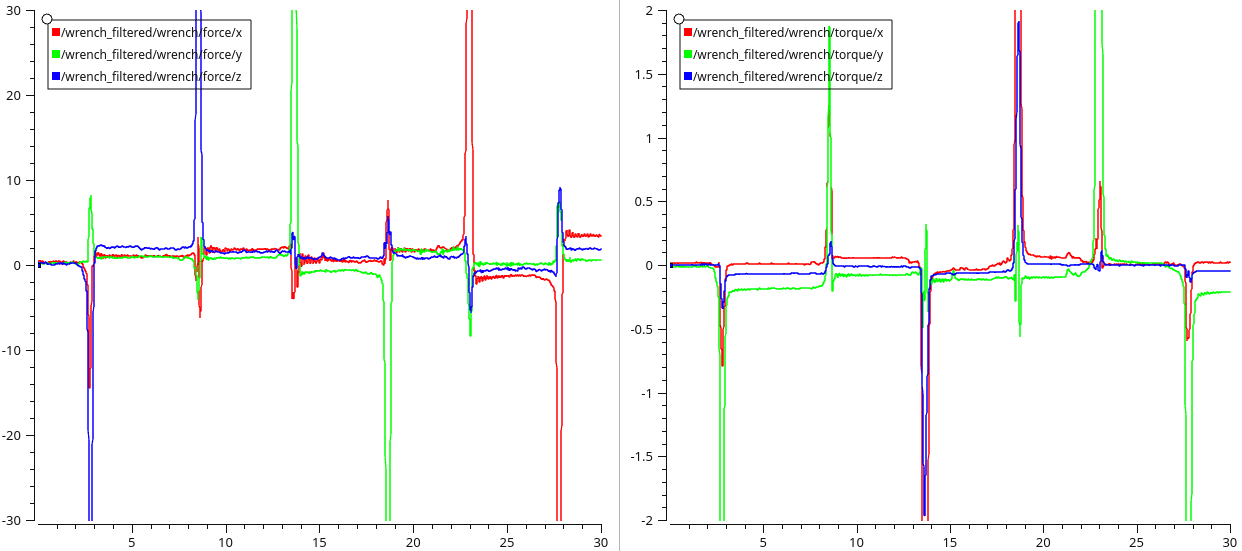
\includegraphics[width=0.9\linewidth]{figs/chp3/ft_sensor_pushes.png}
    \caption{Variation in \ac{ft} relative to interaction with the \ac{eef}}
    \label{fig:ft_sensor_pushes}
\end{figure}

\par Similar to the previous problem, this measurements are wrongly introduced in the system, since the \ac{ft} felt by the sensor should not suffer alterations due to momentarily external interaction with the \ac{eef}.

\subsubsection{Special case of the Z-Axis}

\par Upon coupling a gripper tool to the \ac{eef} of the robot, the force applied by screwing the mounting plate onto the \ac{eef} has effects on the values of force reported on the Z-Axis. The mounting plate has 4 screws, and even making sure they are evenly tightened, the stronger the tightening, the higher the force measurement on the Z-Axis.

\par Measurements of torque in the Z-Axis present momentary fixed variations depending on the amount of movement and direction of the Wrist3 joint. These variations can be seen in any of the real time tests (\autoref{fig:w3_problem}, \autoref{fig:w3_result}, \autoref{fig:ft_theory_result}) but in practicality are irrelevant since they only occur when the robot is moving autonomously, not when the user is applying force to the \ac{eef}.

\subsection{Proposed Solution}
\label{ssec:w3_solution}

\par Regarding the variation of \ac{ft} relative to the Wrist3 joint position, tests were made to prove that the pattern of variation of the measurements was independent of the \ac{eef} orientation, therefore not caused by gravitational forces. The test in question consists on the rotation of the Wrist3 joint from \ang{-360} to \ang{360} in steps of \ang{1}. Each step, the average values of \ac{ft} in a time period of 0.1ms are calculated and saved. The result of the test is a matrix with shape [720, 2, 3], which means 720 values of \ac{ft} in the 3 cartesian axis. The test was performed in each of the 5 positions described in \autoref{fig:eef_5_position}, and its internal behavior can be seen in \autoref{code:w3_test}.

\begin{figure}[h]
    \centering
    \begin{subfigure}{.195\linewidth}
      \centering
      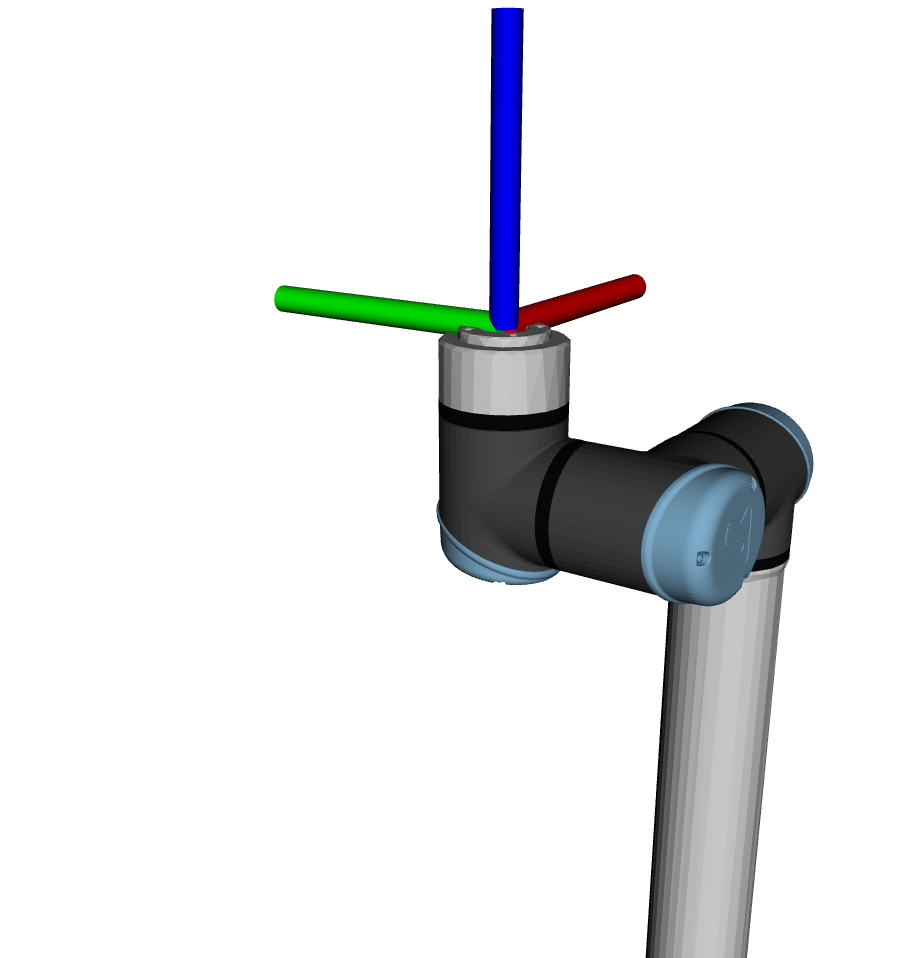
\includegraphics[width=\linewidth]{figs/chp3/P1.png}
      \label{fig:eef_p1}
    \end{subfigure}%
    \begin{subfigure}{.195\linewidth}
      \centering
      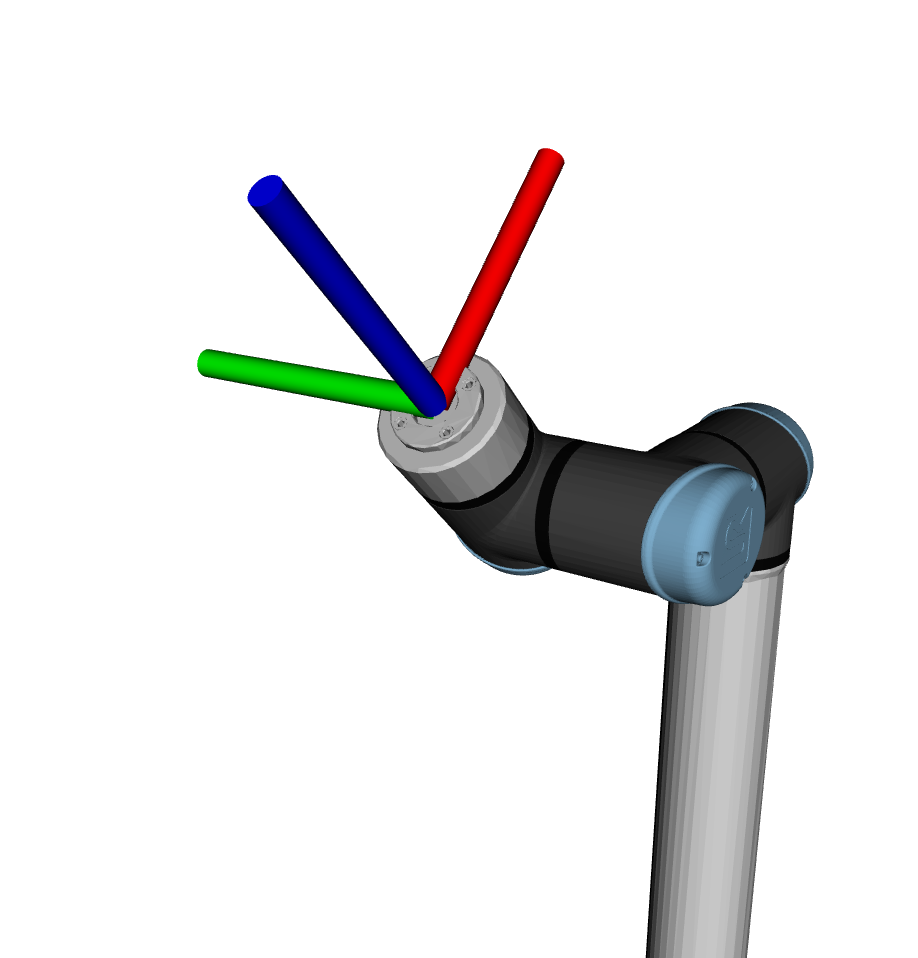
\includegraphics[width=\linewidth]{figs/chp3/P2.png}
      \label{fig:eef_p2}
    \end{subfigure}
    \begin{subfigure}{.195\linewidth}
        \centering
        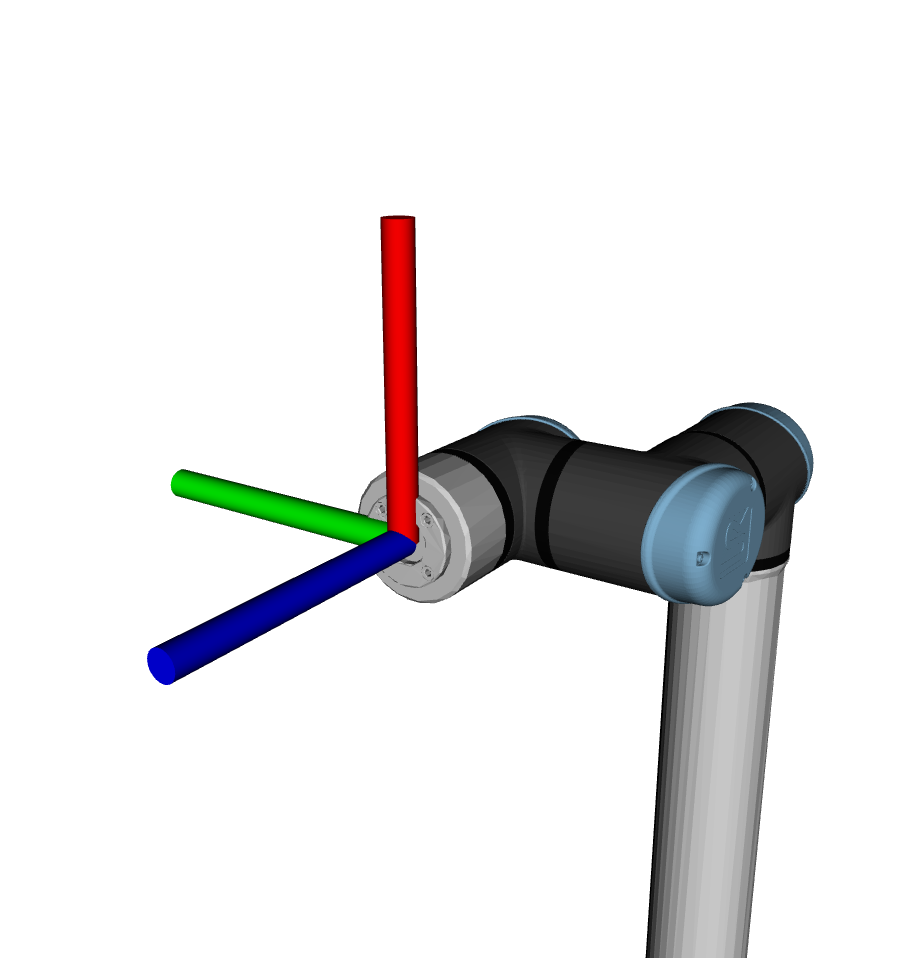
\includegraphics[width=\linewidth]{figs/chp3/P3.png}
        \label{fig:eef_p3}
    \end{subfigure}
    \begin{subfigure}{.195\linewidth}
        \centering
        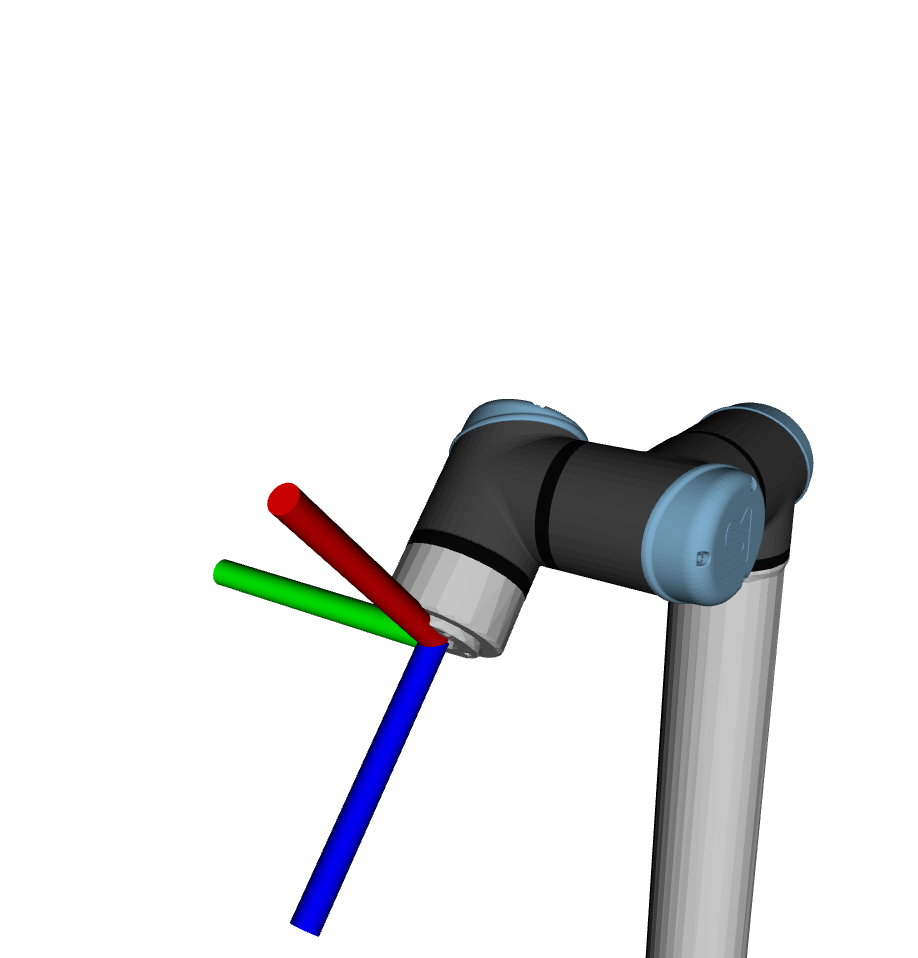
\includegraphics[width=\linewidth]{figs/chp3/P4.png}
        \label{fig:eef_p4}
    \end{subfigure}
    \begin{subfigure}{.195\linewidth}
        \centering
        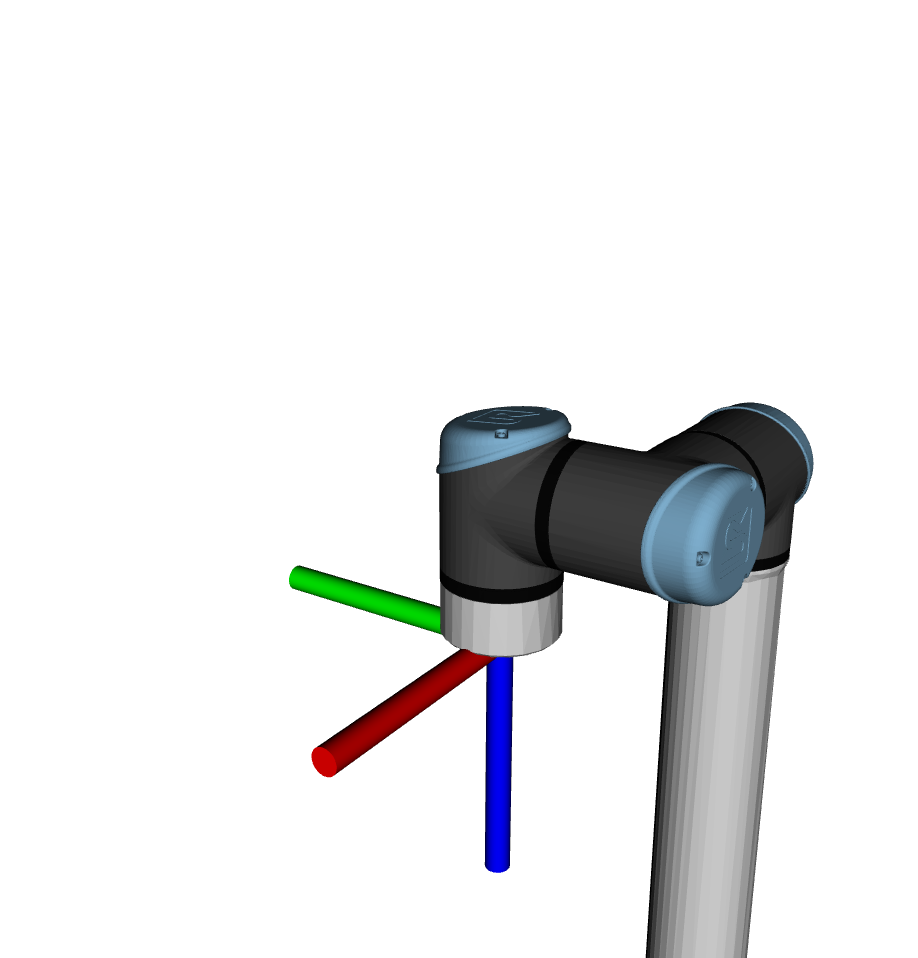
\includegraphics[width=\linewidth]{figs/chp3/P5.png}
        \label{fig:eef_p5}
    \end{subfigure}
    \caption{5 different \ac{eef} testing poses}
    \label{fig:eef_5_position}
\end{figure}

\begin{listing}[h]
    \centering
    \begin{minted}{python}

    wrench = Subscriber("\wrench", size=25)
    
    for pose in poses:
        ur10e.movePose(pose)
        ur10e.zero_ftsensor()
        test = Matrix(720, 2, 3)

        for position in range(-360, 360):
            ur10e.moveWrist3(position)
            sample = wrench.getAverage()
            test.append(sample.force, sample.torque)
        
        saveFile(test)   
    
    \end{minted}
\caption{Recording of \ac{ft} measurements in different poses}
\label{code:w3_test}
\end{listing}

\par The final test results can be seen in \autoref{fig:ft_sensor_test_5}. As predicted, the variation of \ac{ft} only has relation to the position of the Wrist3 joint. Furthermore, the standard deviation of the results is very low, meaning an accurate solution based on the average values recorded can be implemented.

\begin{figure}[h]
    \centering
    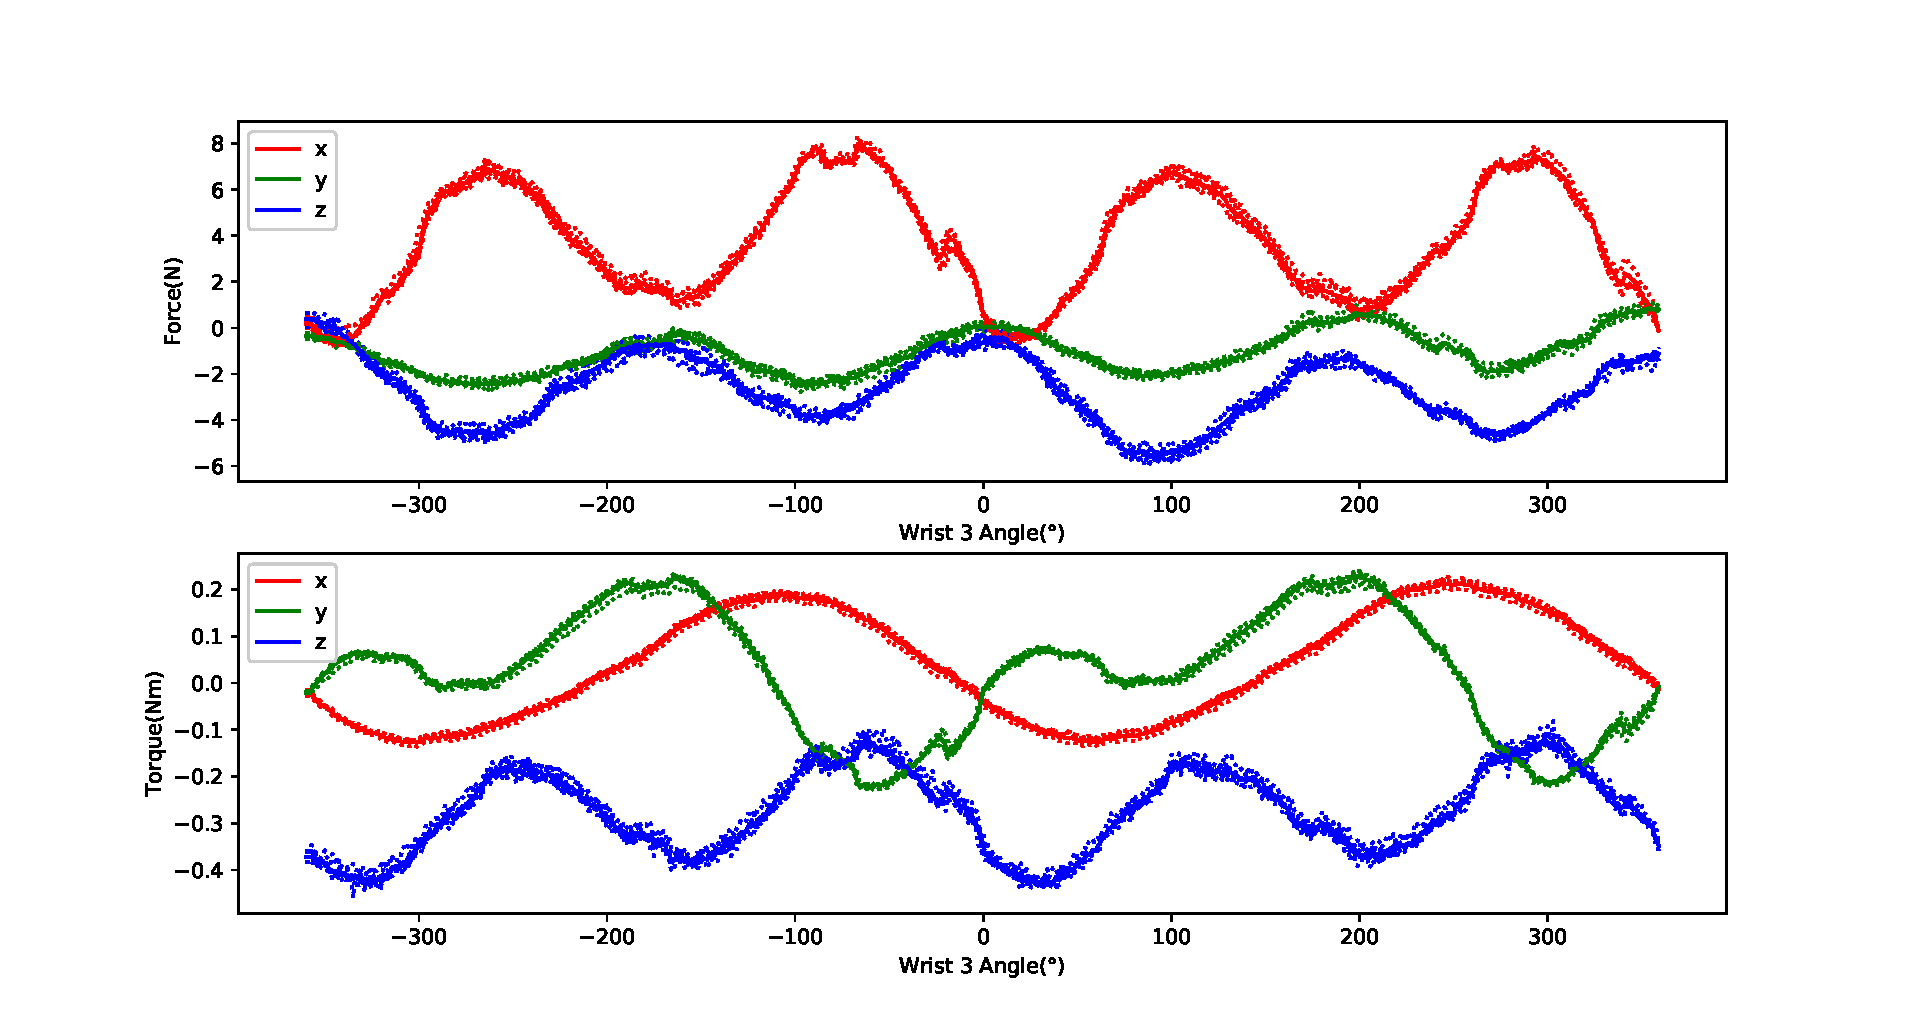
\includegraphics[width=0.8\linewidth]{figs/chp3/ft_sensor_test_5.pdf}
    \caption{Average \ac{ft} values in the 5 testing poses}
    \label{fig:ft_sensor_test_5}
\end{figure}


\par As such, from the average results of the tests performed, a \ac{ros} node was developed to correct in real time the \ac{ft} measurements, based on the position of the Wrist3 joint. It subscribes to the filtered values of \ac{ft} from the topic \textbackslash \textit{wrench\_filtered}, and to the current position of the Wrist3 joint, present in the \textbackslash \textit{joint\_state} topic. The position of the joint serves as index to the correction matrix. The corrected values are published to the \textbackslash \textit{wrench\_corrected} topic.

\par Regarding the variations of \ac{ft} based on time and extreme contacts with the sensor, those problems become irrelevant when a cobot is placed in a real use case scenario. For the drifting problem, a simple idle mode can be implemented, where the robot is suspended if no user or program interacts with it. Once resumed, the \textbackslash\textit{zero\_ftsensor} service can be called, making any \ac{ft} drifting measurements disappear. In the case of the variation of \ac{ft} due to external forces, the solution once again relies on the sensor taring service, since the system can be programmed to trigger it in multiple scenarios, such as a state change or the release of the gripper tool. Further details on the use of this service, in conjunction with a global state machine to solve the inaccuracies of the \ac{ft} sensor are presented in \autoref{chapter:colab-tasks}.

% ADD: Time Series Analysis

\subsection{Results}

\par With the implementation of the correction node, the results from the real time test firstly shown in \autoref{fig:w3_problem} are satisfactory, and presented \autoref{fig:w3_result}.

\begin{figure}[h]
    \centering
    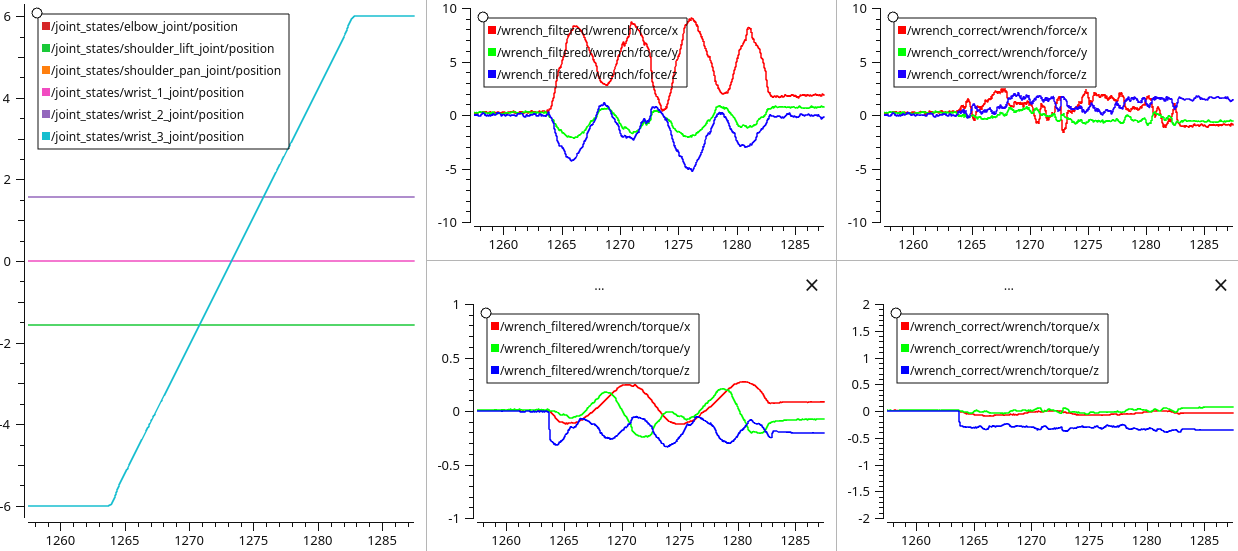
\includegraphics[width=0.9\linewidth]{figs/chp3/wrist_3_result.png}
    \caption{Result of the correction node applied in a real time test}
    \label{fig:w3_result}
\end{figure}

\par The results are as expected. Since the observed pattern is caused by the position of the Wrist3 joint, and is highly repeatable, the corrected \ac{ft} measurements present themselves relatively close to 0 since the \ac{eef} once again has nothing attached. Some variation is still present on the results of \autoref{fig:w3_result}, but it is caused by the nature of the test. Since the movement of the Wrist3 joint is continuos, vibrations and jitters are likely to cause forces on the \ac{eef} that ultimately are caught by the sensor.


\begin{figure}[h]
    \centering
    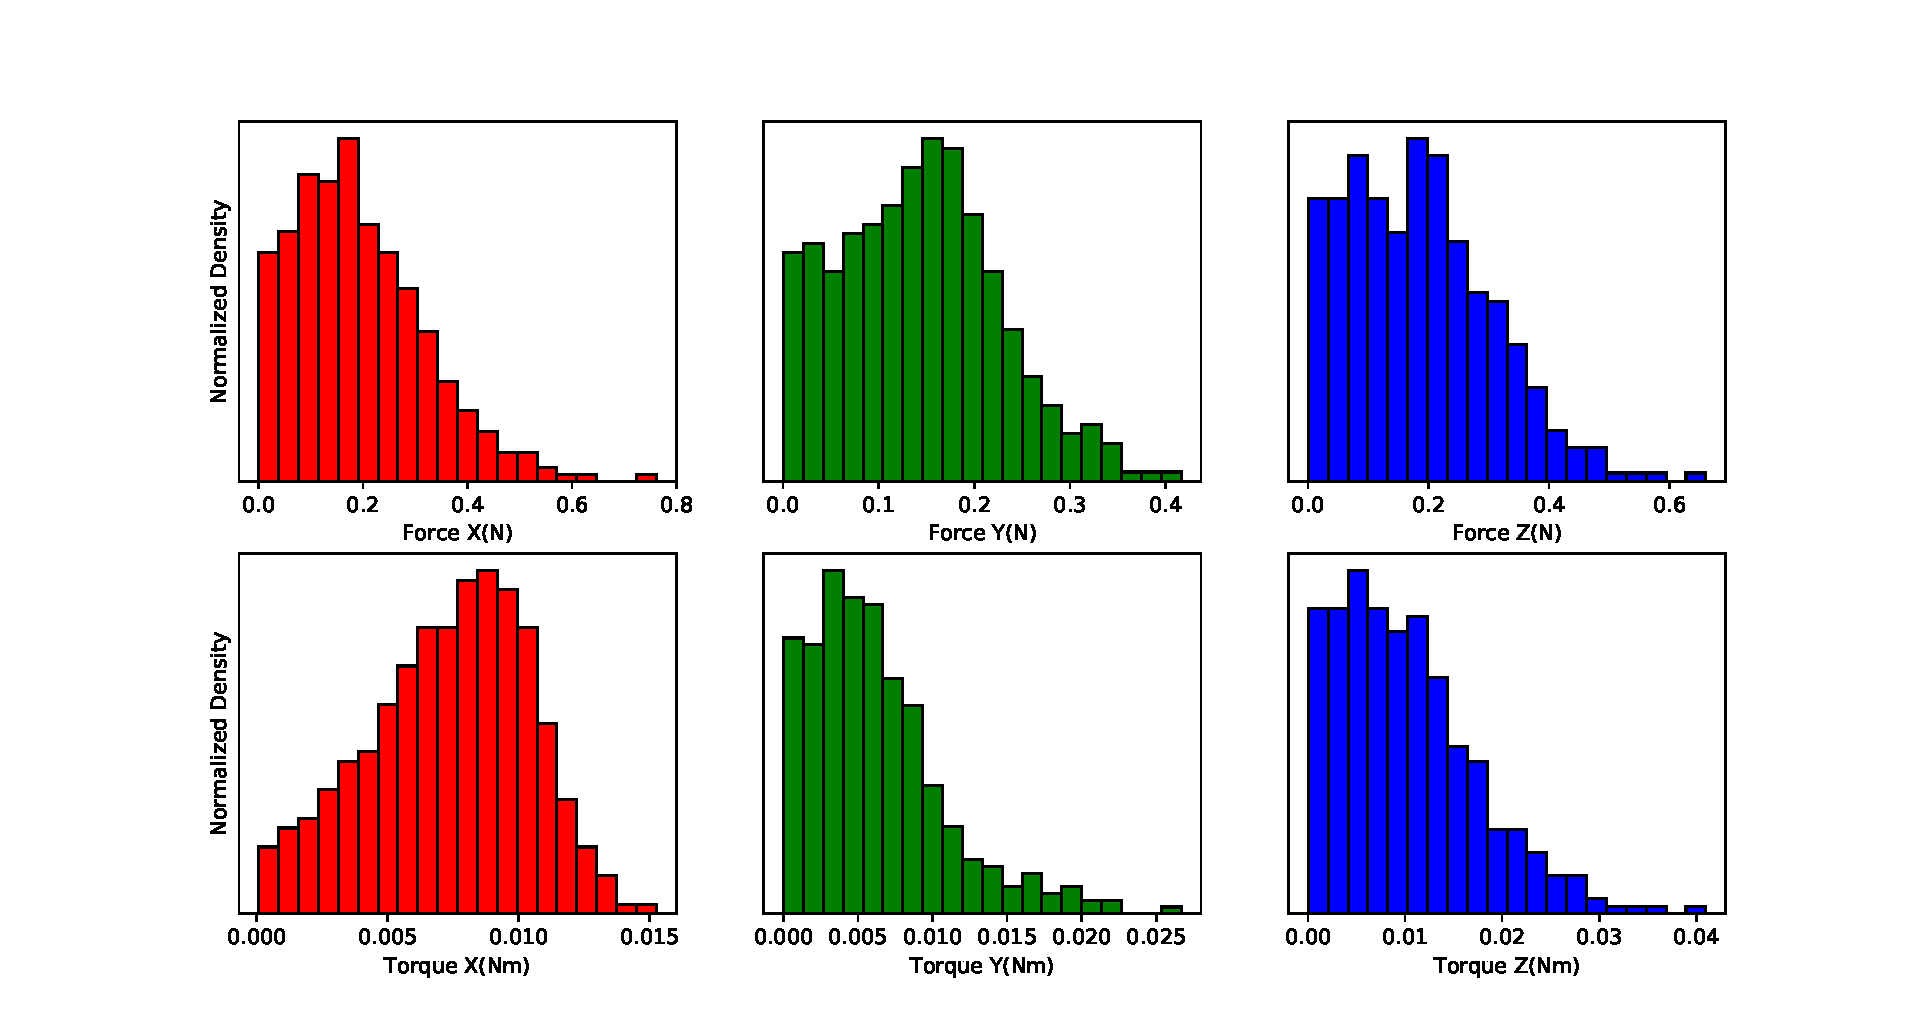
\includegraphics[width=0.8\linewidth]{figs/chp3/wrist_3_result_hist.pdf}
    \caption{Distribution of the correction function error on \ac{ft} measurements}
    \label{fig:w3_result_hist}
\end{figure}

\par A more accurate view on the results obtained is shown in \autoref{fig:w3_result_hist}. Each bar in the histograms represents the probability of the correction error be within that range. The results are considered satisfactory since there is not a single component with an error higher than the resolution specifications of the \ac{ft} sensor (\autoref{tbl:ur10e-specs}).


\section{\ac{eef} Weight Compensation}

\par With the \ac{ft} sensor properly corrected, its measurements can be used for various applications. One of the objectives of this Dissertation is the precise manipulation of heavy objects though \ac{hg}. To do so, there needs to be a way to differentiate \ac{ft} caused by the gravitational forces on the object or tool attached to the \ac{eef}, and \ac{ft} caused by direct physical contact of the user. 


\subsection{\acs{ur} \acs{ft} Sensor Controller Internal Compensation}
\label{ssec:ft_internal_comp}

\par On the Polyscope interface, there is a configuration parameter that directly affects the behavior of the \ac{ft} sensor, called Payload. With this parameter, the user should declare the mass and the \ac{cog} of the object attached to the \ac{eef}. In the previous tests the Payload parameter was configured to zero in the two components. The effects of this configuration parameter can be seen on \autoref{fig:ft_sensor_behavior} where the same positional test was performed, this time with the correction function applied. The Payload parameters for this test were 1.5Kg and a \ac{cog} of 0.1m in the Z-Axis. The \ac{eef} had nothing attached to it.

\begin{figure}[h]
    \centering
    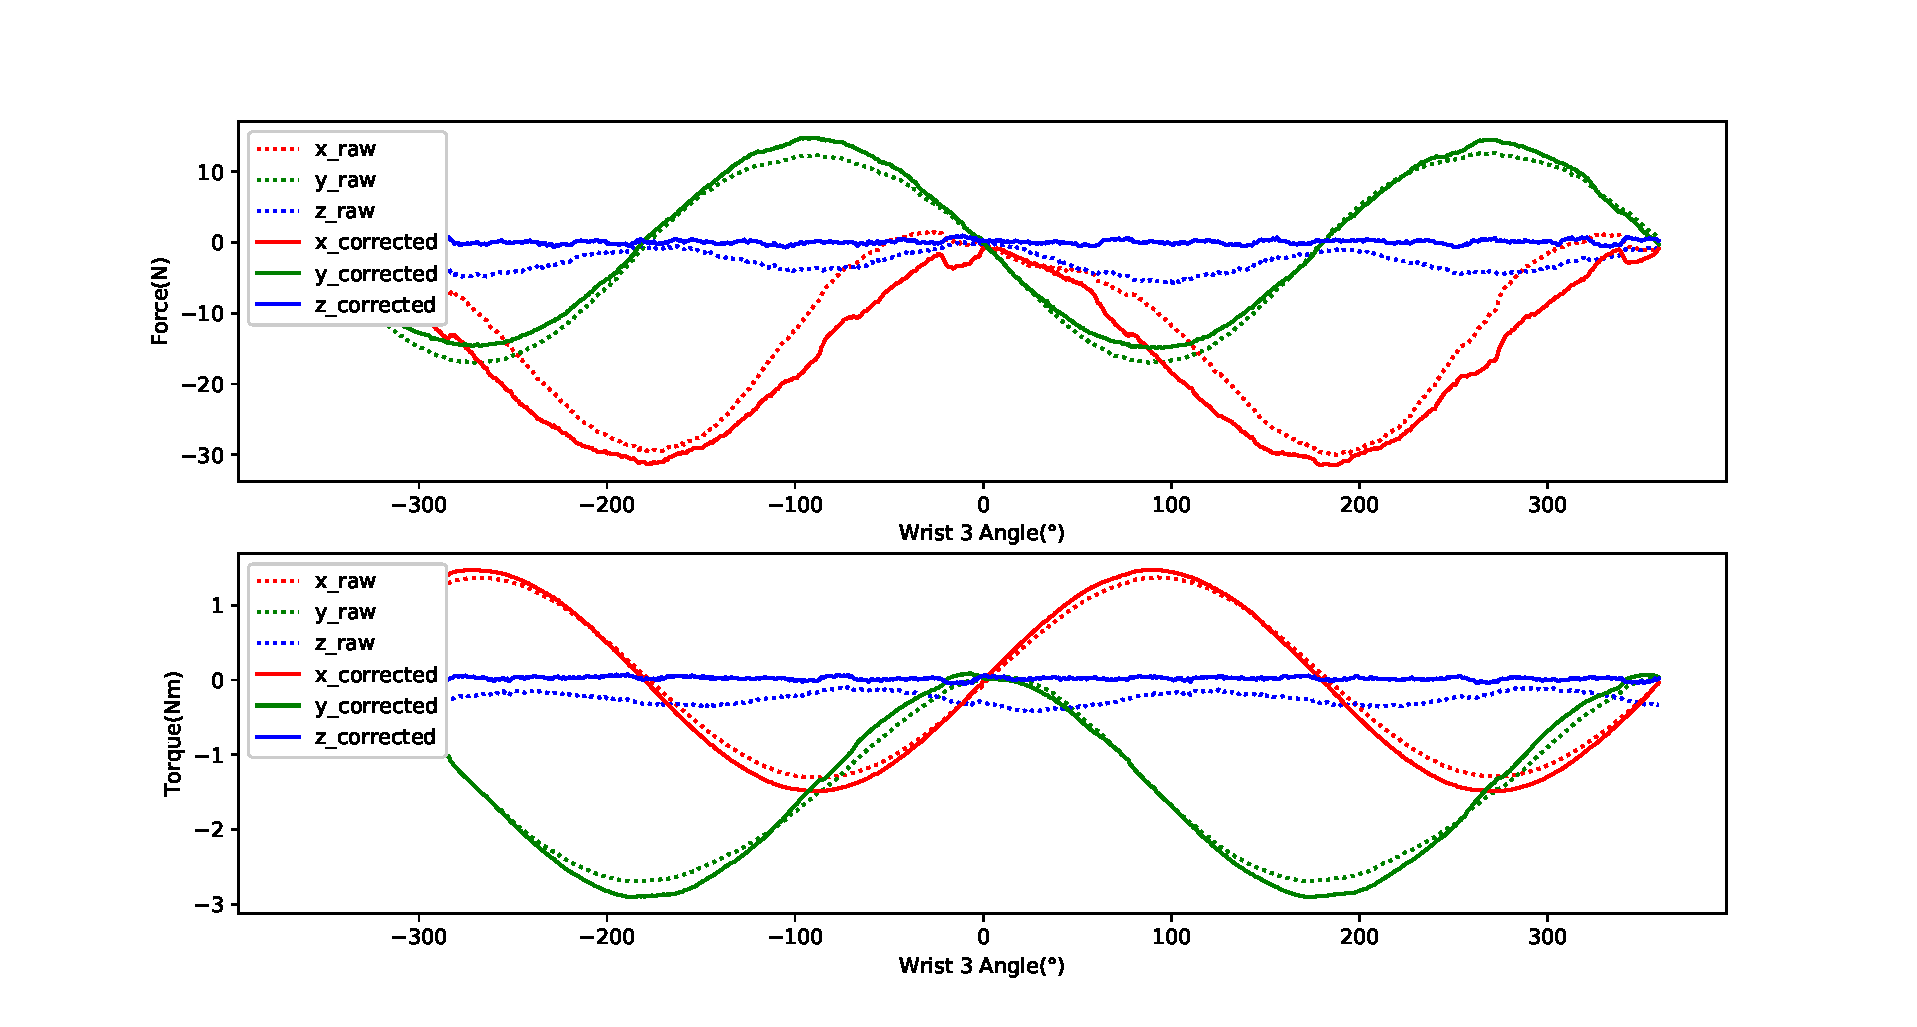
\includegraphics[width=0.8\linewidth]{figs/chp3/ft_sensor_behavior.pdf}
    \caption{Behavior of the FT sensor with parametrization of payload and cog }
    \label{fig:ft_sensor_behavior}
\end{figure}

\par Results show a direct compensation of the configured parameters. In terms of accuracy, the \ac{ft} sensor was tared when the position of Wrist3 joint was \ang{0} and once it rotated to \ang{180}, the force measurement on the X-Axis was $-30\si{N}$, which appears to be correct given the configured mass. Despite this fact, there is no knowledge on the implementation of this compensation mechanism and other tests revealed some inaccuracies on its behavior. Furthermore, the use of this parameter would required its constant update when manipulating objects. The \ac{ros} Driver enables this feature through a service, but every time the Payload parameter is updated, the sensor is tared. 
\par For this reasons, and for the fact that this Payload parameter might not exist in other cobotic platforms or sensors, the chosen values of Payload in this Dissertation are 0, and a theoretical compensation model will be developed with the same objective, but enabling the user to have more control over the use of the \ac{ft} measurements.

\subsection{\acs{ft} Theoretical Model}
\label{ssec:ft_model}

\par The objective of this model is to generate the values of \ac{ft} that a given object or tool would cause on a perfect sensor. This way, when manipulating objects with the cobot, this generated values can be subtracted from the reported sensor measurements and easily obtain the \ac{hgft}. This model is generalized and can be used in any cobot or sensor. As inputs, it requires the orientation of the frame of the \ac{ft} sensor, and the mass and \ac{cog} of the object attached to the \ac{eef}.

\subsubsection{Force}

\par With the orientation of the sensor relative to the world, 3 unit vectors are created representing the measurement cartesian components. Then, calculating the theoretical force is done with using the inner product of a unit vector representing gravity, and each one of the cartesian unit vectors. \autoref{fig:ft_theory_force} shows a visual representation of such method.

\begin{figure}[h]
    \centering
    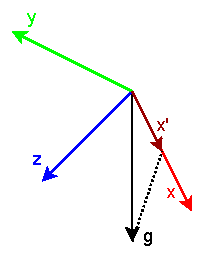
\includegraphics[width=0.3\linewidth]{figs/chp3/ft_theory_force.pdf}
    \caption{Visualization of the generation of theoretical force values}
    \label{fig:ft_theory_force}
\end{figure}

\begin{figure}[h]
    \begin{equation}
        \mathbf{Fx} = \langle \hat{x_{eef}} , \hat{g} \rangle \cdot m \cdot g
        \label{eq:theory_force}
    \end{equation}
\end{figure}

\par \autoref{eq:theory_force} generates the force in the X-Axis where $\mathbf{\hat{x_{eef}}}$ represents a unit vector with the orientation of the X-Axis in the \ac{ft} sensor frame, $\mathbf{\hat{g}}$ is a unit vector representing gravity, $\mathbf{m}$ is the mass of the object and $\mathbf{g}$ the acceleration of gravity.

\subsubsection{Torque}

\par Analogous to the generation of forces, torque generation also relies on the representation of the cartesian axis as unit vectors. This time, a new vector containing the direction and magnitude of the theoretical torque is created using the cross product of gravity and the \ac{cog} of the object. With this vector, torque in each axis can be calculated with the inner product, just like in the force generation. For a better understanding, \autoref{fig:ft_theory_torque} shows a visual representation of this method.

\begin{figure}[h]
    \centering
    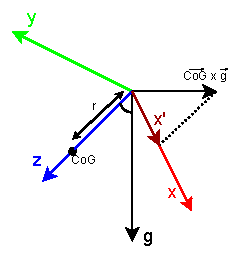
\includegraphics[width=0.35\linewidth]{figs/chp3/ft_theory_torque.pdf}
    \caption{Visualization of the generation of theoretical torque values}
    \label{fig:ft_theory_torque}
\end{figure}

\begin{figure}[h]
    \begin{equation}
        \mathbf{Tx} = \langle\hat{x_{eef}} , \vec{CoG} \times \vec{g} \rangle \cdot m \cdot g\cdot r
        \label{eq:theory_torque}
    \end{equation}
\end{figure}

\par \autoref{eq:theory_torque} generates the torque in the X-Axis where $\mathbf{\hat{x_{eef}}}$ represents a unit vector with the orientation of the X-Axis, $\mathbf{\vec{CoG}}$ represents a unit vector with the orientation of the \ac{cog}, $\mathbf{\hat{g}}$ is a unit vector representing gravity, $\mathbf{m}$ is the mass of the object, $\mathbf{g}$ the acceleration of gravity and $\mathbf{r}$ is the distance of the \ac{cog} to the origin.

\subsection{Results}
\label{ssec:ft_theory_results}

\par To test the accuracy of the model, the Wrist3 joint test was performed with a gripper tool attached to the \ac{eef}. The weight of the tool is 1.5Kg and its \ac{cog} is 0.045m in the Z-Axis. While the test was executing, the values from the theoretical model and the real \ac{ft} sensor were recorded and can be seen in \autoref{fig:ft_sensor_theory}.

% ADD: Describe how to the CoG was obtained for the gripper

\begin{figure}[h]
    \centering
    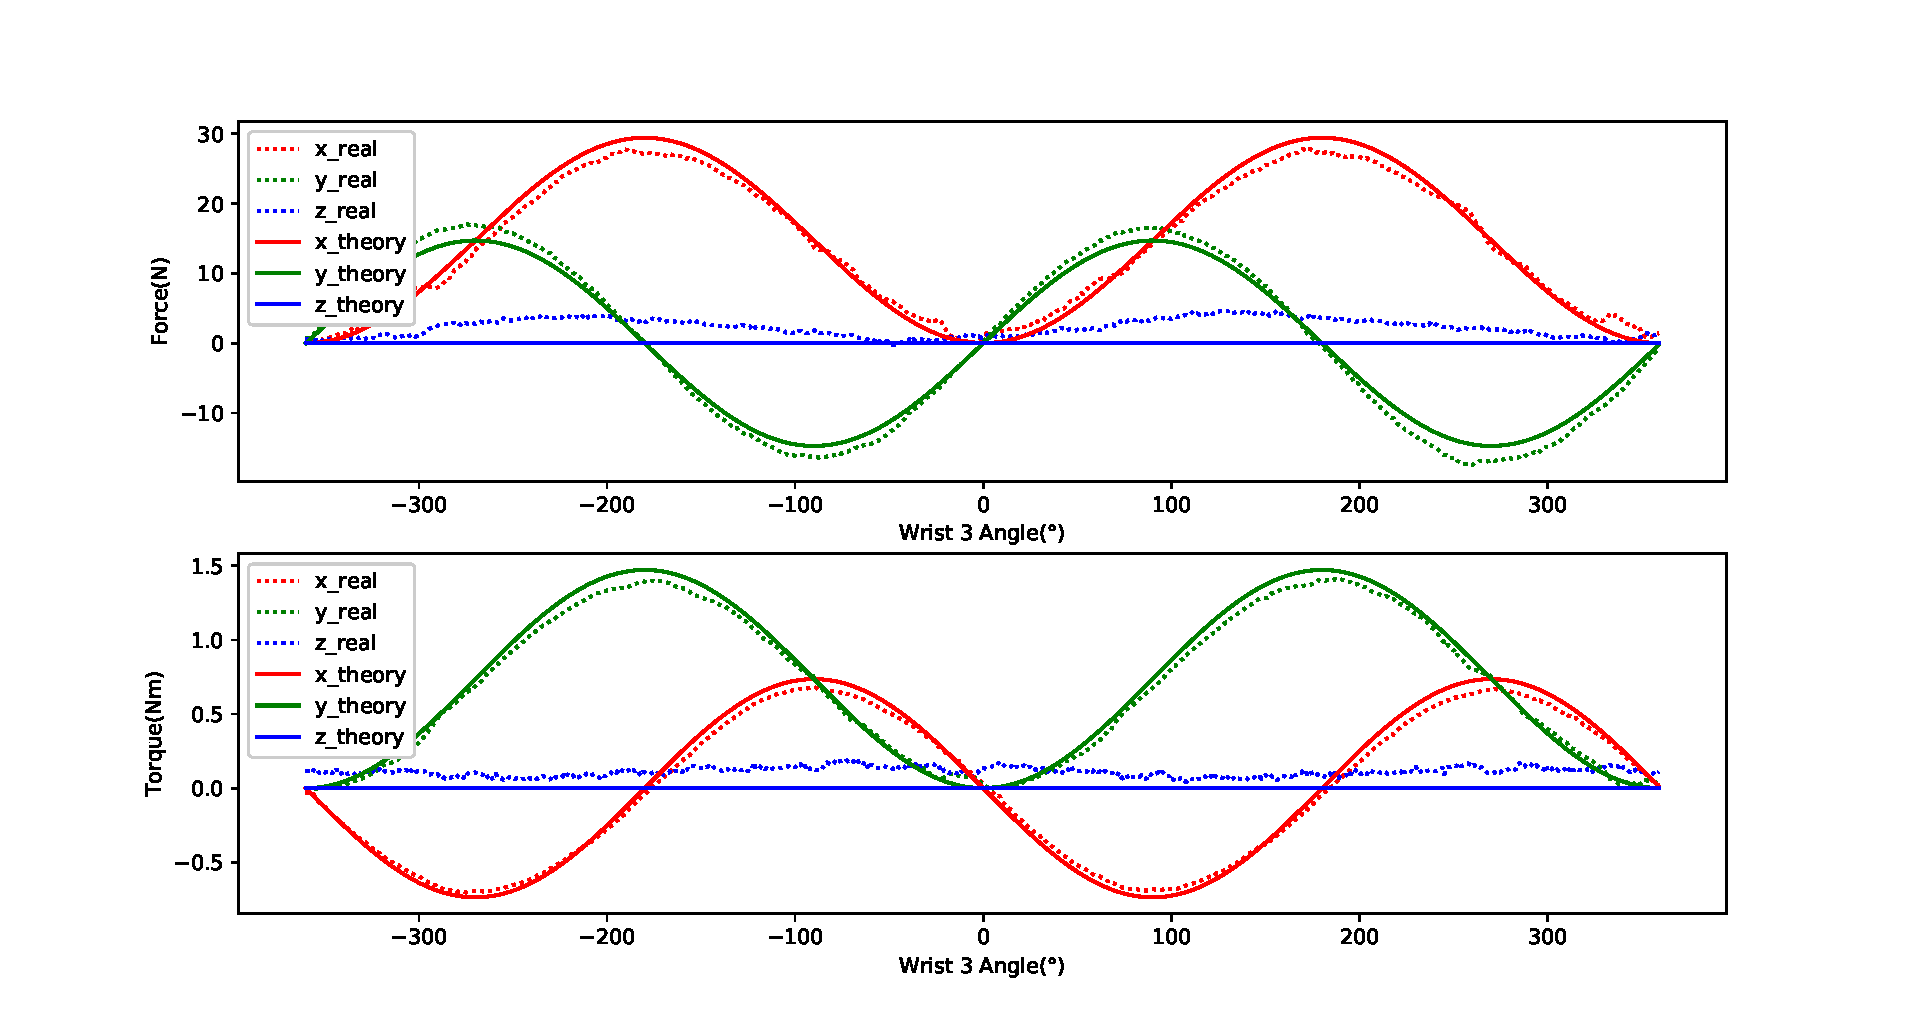
\includegraphics[width=0.8\linewidth]{figs/chp3/ft_sensor_theory.pdf}
    \caption{Comparison of \ac{ft} measurements from real sensor and analytical model}
    \label{fig:ft_sensor_theory}
\end{figure}

\par Regarding force generation, X-Axis and Y-Axis real measurements appear to deviate from the analytical values by a constant factor. Because this factor is higher than 1 in the Y-Axis and lower than 1 on the X-Axis, it is not caused by the weight parameter, but rather by the internal behavior of the \ac{ft} sensor. In the case of the Z-Axis, there are large deviations from the analytical model and it appears to be influenced by the force in the X-Axis.
% Z-Axis might also be influenced negatively by Y-Axis
\par Regarding torque generation, both X-Axis and Y-Axis appear accurate. The offset that exists in the Z-Axis is caused by the nature of the test, since it consists on successive rotations of the Wrist3 joint, where the \ac{ft} sensor is located.

\begin{figure}[h]
    \centering
    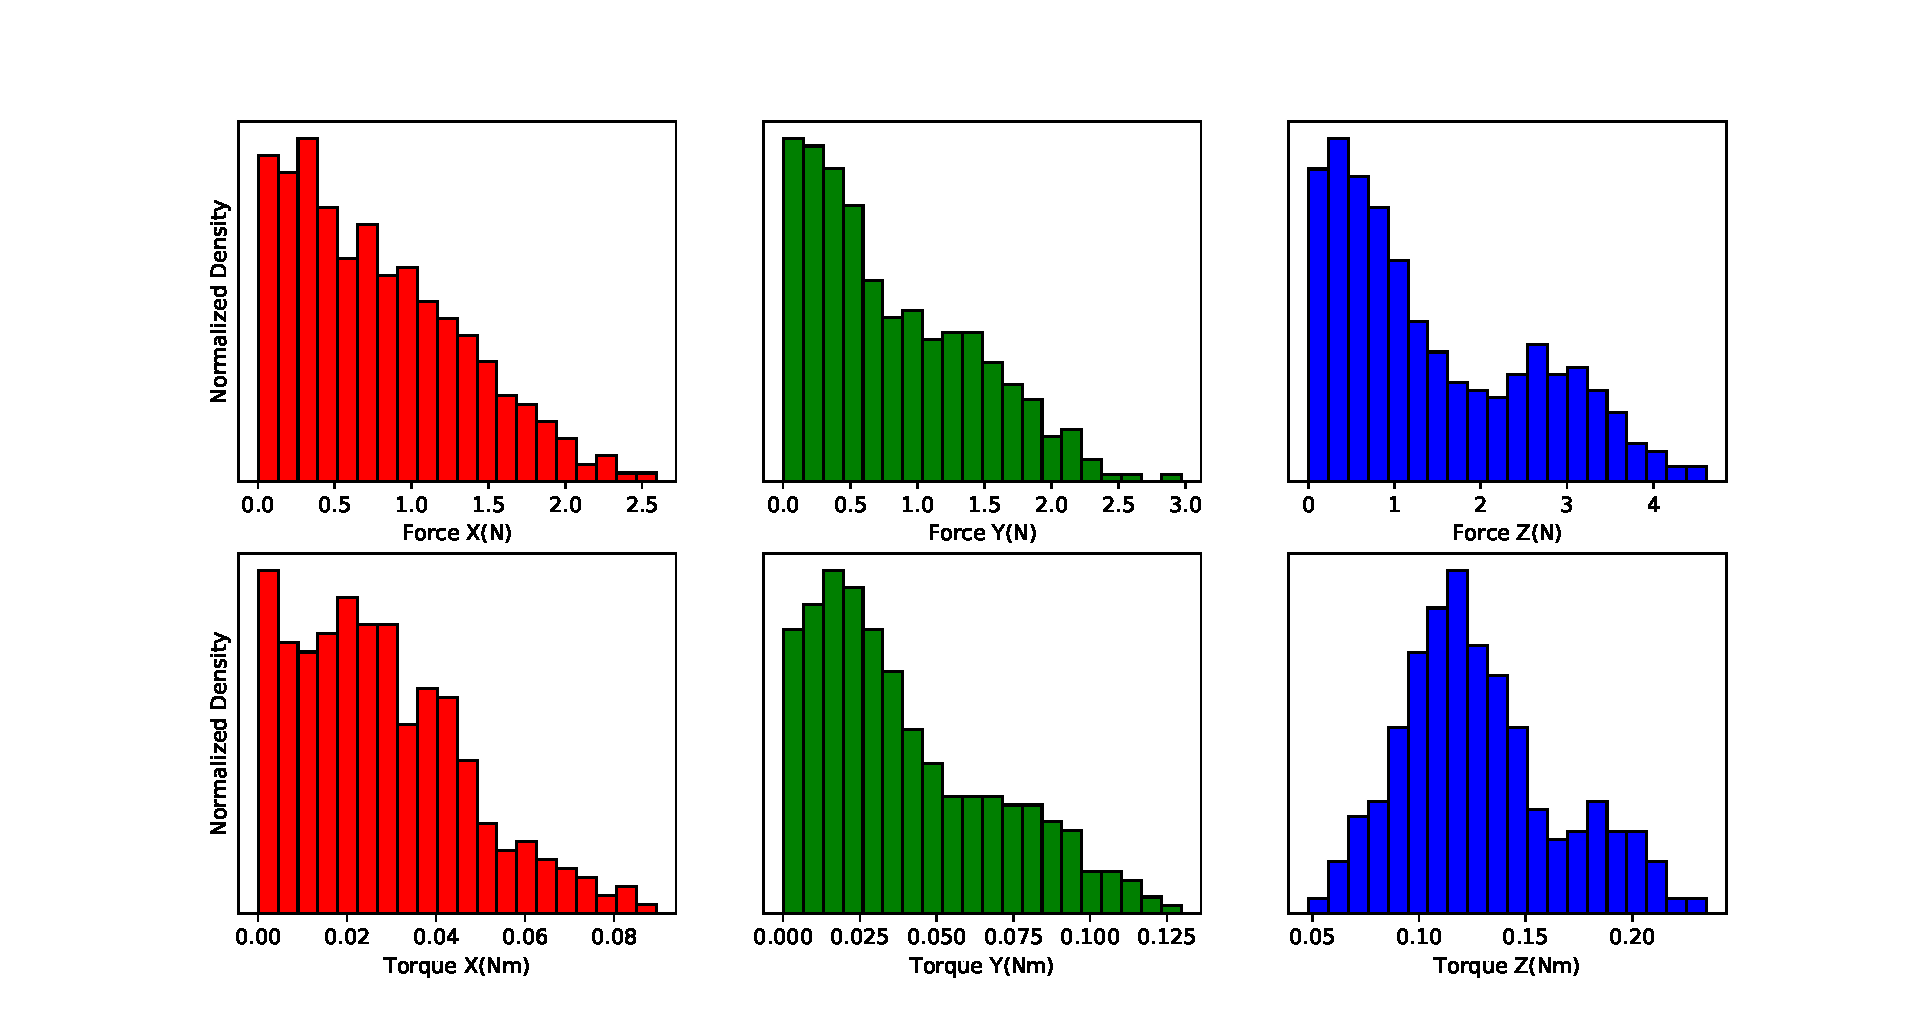
\includegraphics[width=0.8\linewidth]{figs/chp3/ft_sensor_theory_hist.pdf}
    \caption{Distribution of analytical model error on \ac{ft} measurements}
    \label{fig:ft_sensor_theory_hist}
\end{figure}

\par Once again, a probabilistic view in the form of histograms can better help understand the accuracy of the model. \autoref{fig:ft_sensor_theory_hist} shows that for X-Axis and Y-Axis, the \ac{ft} error is well below the accuracy specification of the sensor (\autoref{tbl:ur10e-specs}). For the Z-Axis, despite also being below the accuracy specification, it is significantly higher than the other 2 components and can damage the precision of an \ac{hg} task, since the \ac{ft} threshold must be higher than the error of the least accurate component. Given this fact efforts were made to adapt the analytical model to better match the real values. 

\subsection{Adapting the \ac{ft} Theoretical Model}

% ADD: Melhorar a parte prática desta secção com mais testes e fazer com que eles sejam dependentes de W1 e W2

\par By running tests in a variety of different \ac{eef} orientations, both real and analytical measurements can be compared and the deviation factors can be computed. Since the the positional test relies on the movement of the Wrist3 joint, in order to create different \ac{eef} poses, a combination of Wrist1 and Wrist2 joints angles was used. With steps of \ang{45} between \ang{-180} and \ang{180}, a total of 57 different poses can be achieved by combining these 2 wrist joints. \autoref{fig:57_poses} is a visualization of the resulting \ac{eef} orientations.

\begin{figure}[h]
    \centering
    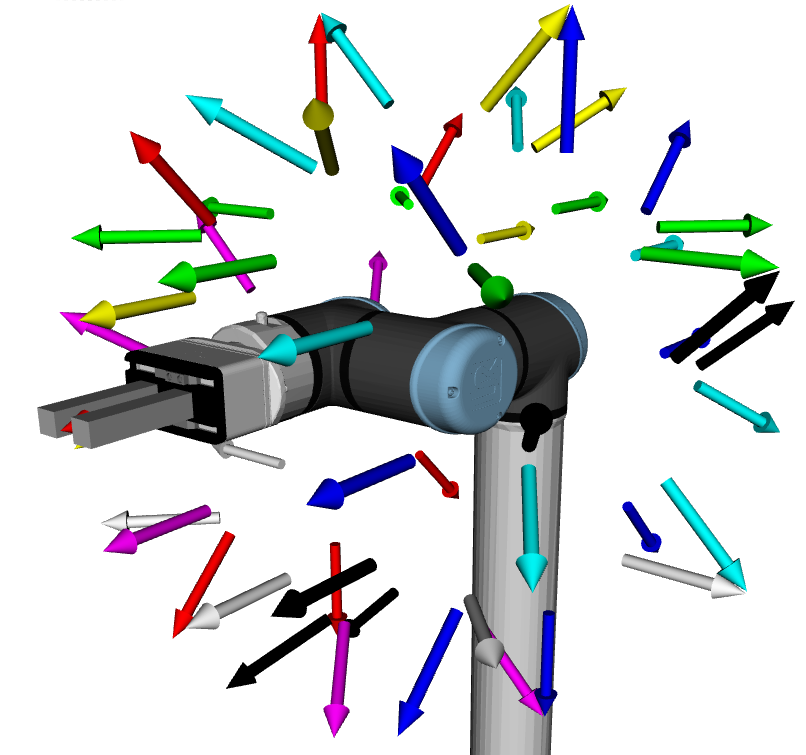
\includegraphics[width=0.35\linewidth]{figs/chp3/globe_57.png}
    \caption{Visualization of the 57 poses in which the tests were performed}
    \label{fig:57_poses}
\end{figure}

\par In each orientation, a Wrist3 positional test is performed, recording both analytical and real \ac{ft} measurements. With the results, an optimization function based on the \ac{dls} method is used to find the deviation coefficients between the analytical and real measurements. After obtaining such coefficients, they are inserted in the analytical model as correction factors of the generated values. When performing the same tests as in \autoref{ssec:ft_theory_results}, the difference between the analytical and real measurements is reduced, and the error is now in the range of the noise generated by the sensor, allowing for greater precision in \ac{ft} dependant tasks.

\begin{figure}[h]
    \centering
    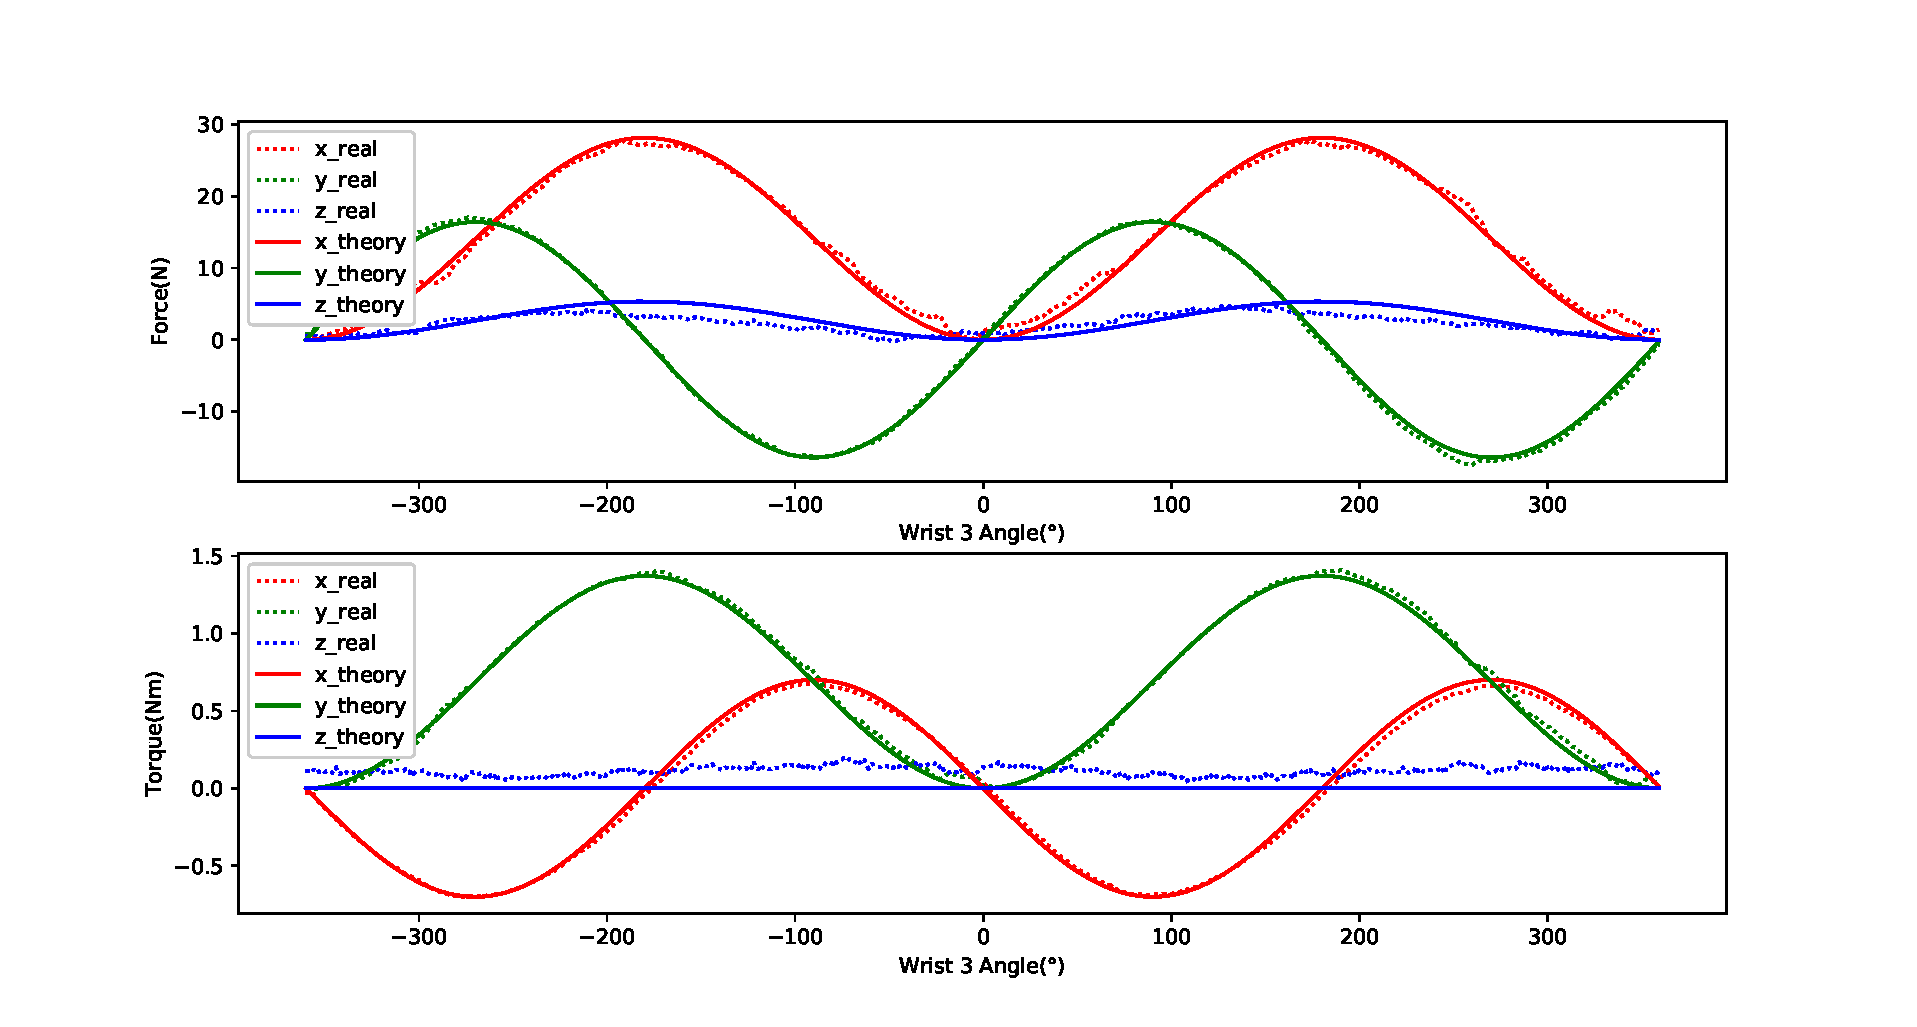
\includegraphics[width=0.8\linewidth]{figs/chp3/ft_sensor_theory_adjust.pdf}
    \caption{Comparison of \ac{ft} measurements from real sensor and adjusted analytical model}
    \label{fig:ft_sensor_theory_adjust}
\end{figure}

\par This fact is shown in \autoref{fig:ft_sensor_theory_adjust} where \ac{ft} analytical and real measurements appear overlapped. Futhermore, \autoref{fig:ft_sensor_theory_adjust_hist} details the distribution of the errors between the 2 measurements and shows what threshold interaction \ac{ft} values can be used in an \ac{hg} task. Given the observations, it is safe to say that a force threshold of 2N and a torque threshold of 0.2Nm are possible. These are very low amounts of \ac{ft} and a system that can react to them allows precision and ease of use in any sort of manipulation task.

\begin{figure}[h]
    \centering
    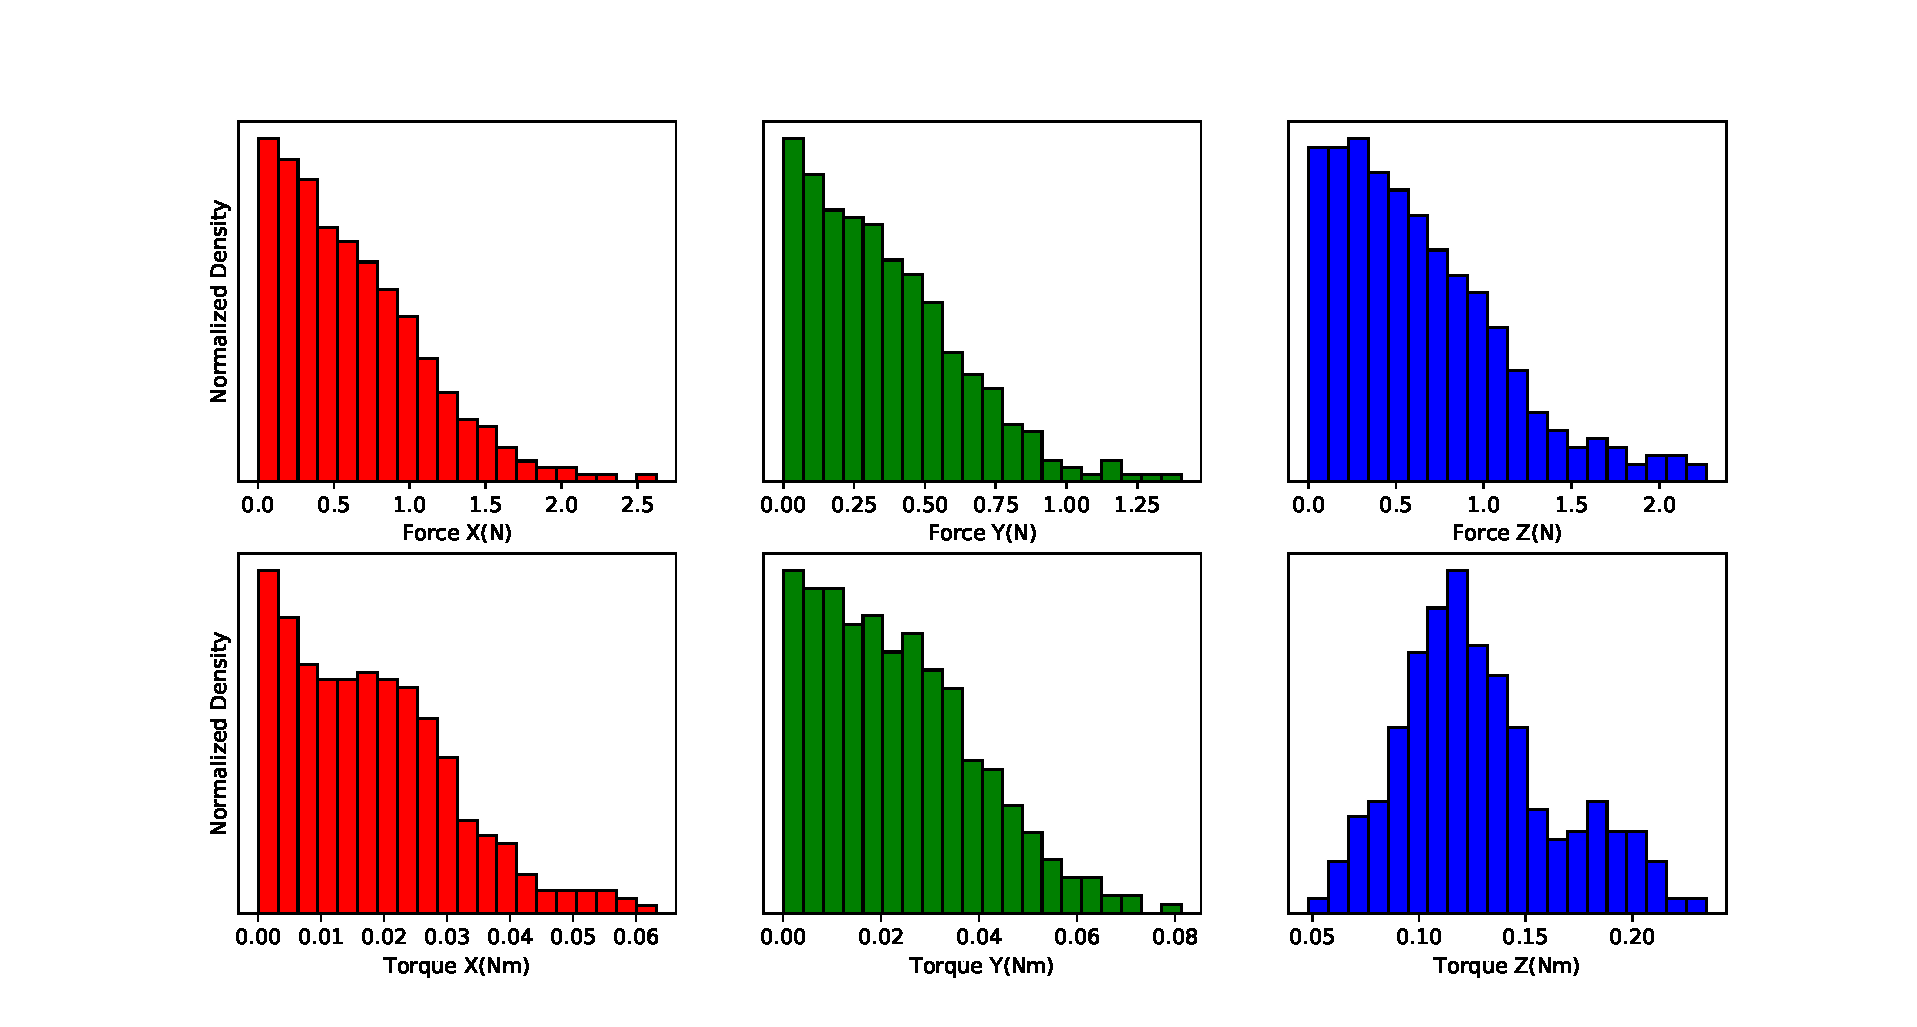
\includegraphics[width=0.8\linewidth]{figs/chp3/ft_sensor_theory_adjust_hist.pdf}
    \caption{Distribution of the adjusted analytical model error on \ac{ft} measurements}
    \label{fig:ft_sensor_theory_adjust_hist}
\end{figure}

\subsection{Real Time Correction and Compensation of \ac{ft}}

\par In order to obtain the corrected and compensated \ac{ft} measurements in real time, a group of \ac{ros} nodes were developed. Some of them were already previously explained such as the Driver, Filter and Correct nodes. These nodes were arranged together according to the architecture described in \autoref{fig:ft_ros_arch}.

\begin{figure}[h]
    \centering
    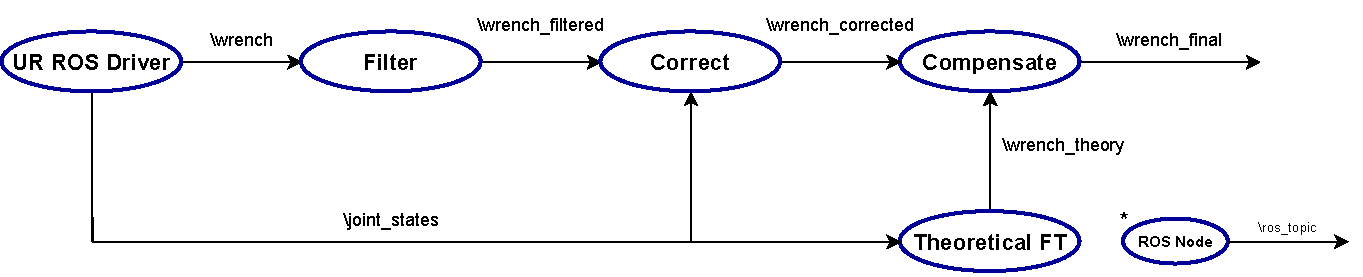
\includegraphics[width=\linewidth]{figs/chp3/ft_comp_ros_arch.pdf}
    \caption{ROS architecture of the compensation of \ac{ft} in real time}
    \label{fig:ft_ros_arch}
\end{figure}

\par The Theoretical FT node implements the algorithms explained in \autoref{ssec:ft_model}. It subscribes to the state of the \ac{ur10e} in order to obtain the \ac{eef} pose. Then calculates the theoretical \ac{ft} values and publishes them to the \textbackslash\textit{wrench\_theory} topic. This node has 2 internal parameters, "weight" and "cog" that can be updated both from the dynamic reconfigure \ac{ros} tool and from a \ac{ros} service named \textbackslash\textit{cobot}\textbackslash\textit{payload\_update}.
\par Finally, the Compensate node subscribes to both the corrected and analytical values, and publishes the final \ac{ft} measurements. It provides a \ac{ros} service called \textbackslash \textit{cobot}\textbackslash\textit{zero\_ftsensor} used to synchronize the corrected and analytical values when the user wants to zero the \ac{ft} sensor. This is the recommended way to intentionally tare de \ac{ft} sensor, since this way, previous information is not lost and the remaining nodes dependent of this values, can interoperate safely.

\begin{figure}[h]
    \centering
    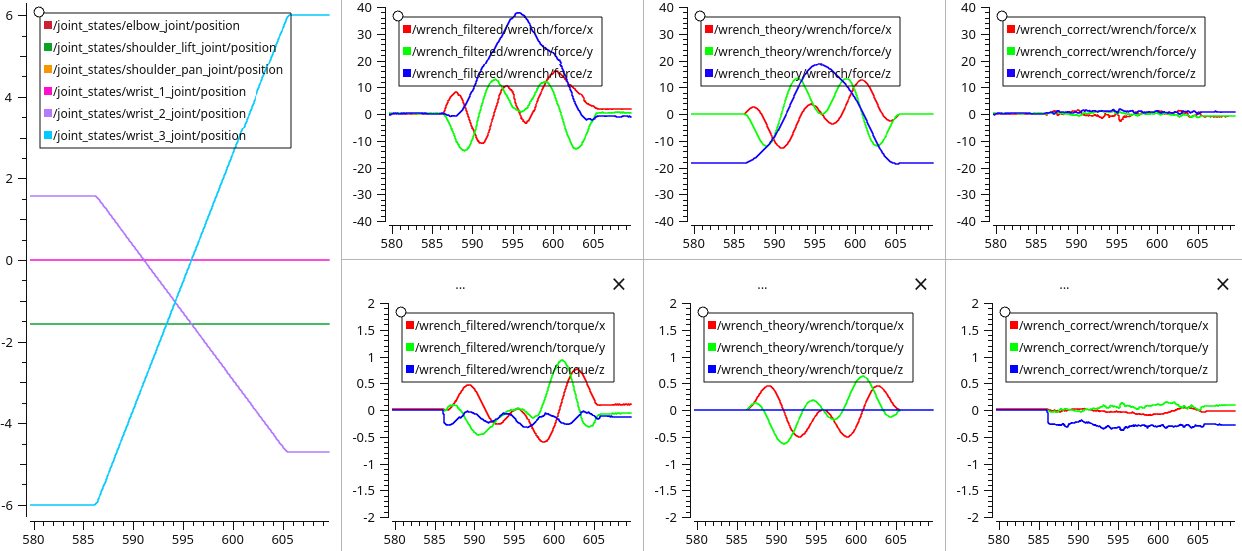
\includegraphics[width=0.9\linewidth]{figs/chp3/ft_sensor_theory_result.png}
    \caption{Result of the compensation architecture applied in a real time test}
    \label{fig:ft_theory_result}
\end{figure}

\par To test this architecture, a real time test was performed where multiple joints were rotated to provoque various orientations on the \ac{eef}, which had a gripper tool attached to it. \autoref{fig:ft_theory_result} demonstrates the execution and results of this test, where the Wrist2 and Wrist3 joints are simultaneously rotated. The graphs in the middle show both the real and analytical \ac{ft} measurements. Their subtraction results in the final \ac{ft} measurements, shown in the leftmost graphs, and since no external \ac{ft} was applied during this test, are all close to 0.
\par This architecture allows for correct separation of \ac{ft} caused by gravitational forces on the attached weight and \ac{ft} caused by human physical interaction. This way, the cobot can have any tool or object attached, and simultaneously be manipulated by the user.

% ADD: Automatic calibration of attached tool and theoretical model
